\documentclass{article}
\title{The off-chain reporting protocol}
\subtitle{An overview of the Chainlink OCR protocol.}

\date{2024-01-30}
\modified{2024-01-30}

\keyword{chainlink}

\begin{document}
\section{abstract}{Abstract}

This article is a high-level overview of the Off-Chain Reporting protocol (\sc{ocr}) powering most of \href{https://chain.link/}{Chainlink} products.
The protocol allows a group of \math{n} nodes called \emph{oracles}, up to \math{f} of which could be \href{https://en.wikipedia.org/wiki/Byzantine_fault}{byzantine} (\math{f < n⁄3}), to agree on a data point and record it on a blockchain supporting smart contracts (e.g., Ethereum).

\section{components}{Protocol components}

All \sc{ocr} deployments have two parts with different execution models: the on-chain part, implemented as a smart contract called the \emph{aggregator}, and the off-chain part, implemented as a peer-to-peer network of oracles.
The off-chain communication protocol, in turn, consists of three sub-protocols layered on top of one another: the \href{#pacemaker}{pacemaker}, the \href{#report-generation}{report generation}, and the \href{#transmission}{transmission} protocols. 

\subsection{aggregator-contract}{The aggregator contract}

The aggregator contract is deployed on the blockchain and serves multiple roles:
\begin{enumerate}
    \item It stores the oracle network configuration, such as public keys of nodes participating in the protocol and report generation parameters.
    \item It records the oracle network's reports on the blockchain and makes them available to other smart contracts.
    \item It distributes rewards to the oracles signing and transmitting reports.
\end{enumerate}

The contract owner has administrative privileges, such as adding or removing nodes from the network, changing billing settings, and updating the report generation configuration.

\subsection{pacemaker}{Pacemaker}

The \emph{pacemaker} algorithm of the \sc{ocr} protocol periodically assigns a node to be a \emph{leader} coordinating the rest of the protocol functions.
The period between two consecutive leader assignments is called an \emph{epoch}.
Within each epoch, the leader initiates \emph{rounds} of the \href{#report-generation}{report generation} algorithm.
The tuple \math{(e, r)}, where \math{e} is the epoch number and \math{r} is the round number, serves as a logical clock for the protocol.

\begin{figure}[grayscale-diagram]
    \marginnote{mn-figure-pacemaker}{
        Leader rotation in the pacemaker algorithm.
        Note that the leader is also a follower.
    }
    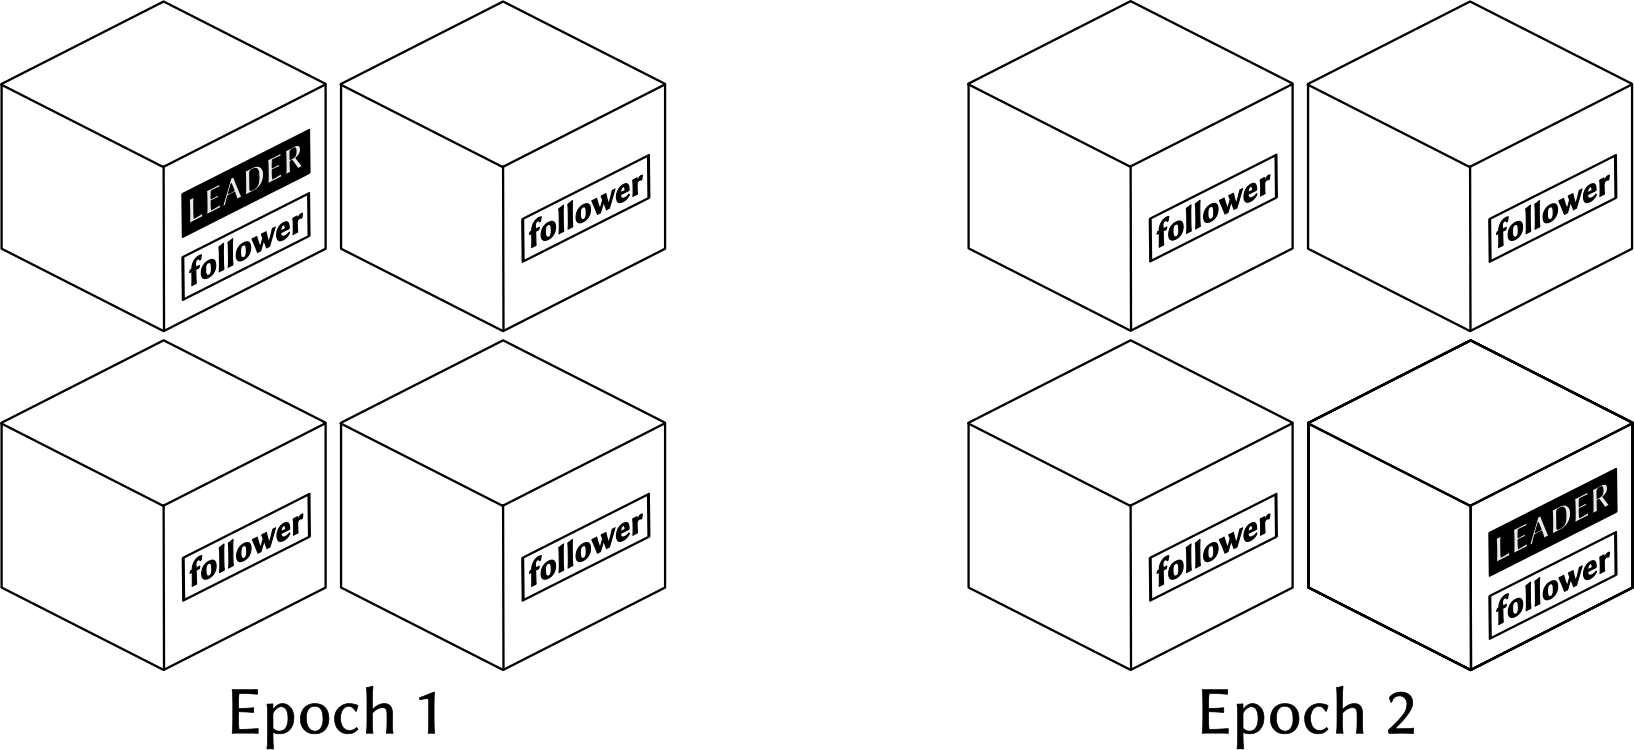
\includegraphics{/images/24-pacemaker.svg}
\end{figure}

The protocol can advance the epoch in two circumstances:
\begin{enumerate}
    \item The current epoch duration exceeded the configured time amount.
    \item The protocol didn't progress for the configured time amount.
\end{enumerate}

The function mapping epoch numbers to leader nodes is a \href{https://crypto.stanford.edu/pbc/notes/crypto/prf.html}{cryptographic pseudo-random function} parameterized by a secret key (called the \emph{seed} key) known only to the oracles.
Thus, oracles know the exact sequence of all leader assignments in advance, but to all outside observers, the assignments are indistinguishable from random.

\subsection{report-generation}{Report generation}

The report generation algorithm produces a data point for the \href{#aggregator-contract}{aggregator contract}.
For example, if the aggregator contract records an asset price in \sc{usd}, the algorithm produces a price that faulty oracles can't manipulate.

First, the leader initiates a new round by picking a \emph{query} describing the task the followers need to execute and sending it to all the followers.
\begin{figure}[grayscale-diagram,medium-size]
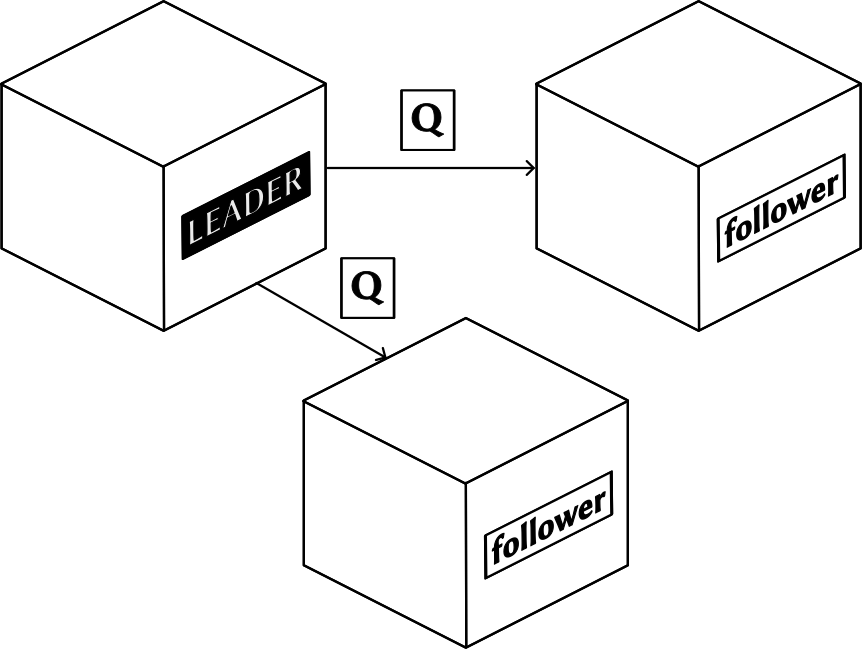
\includegraphics{/images/24-report-1.svg}
\end{figure}

The followers execute the query (usually by observing an external data source) and send a signed \emph{observation} back to the leader.
In the asset price example, the observation will be their guess of the asset price.
\begin{figure}[grayscale-diagram,medium-size]
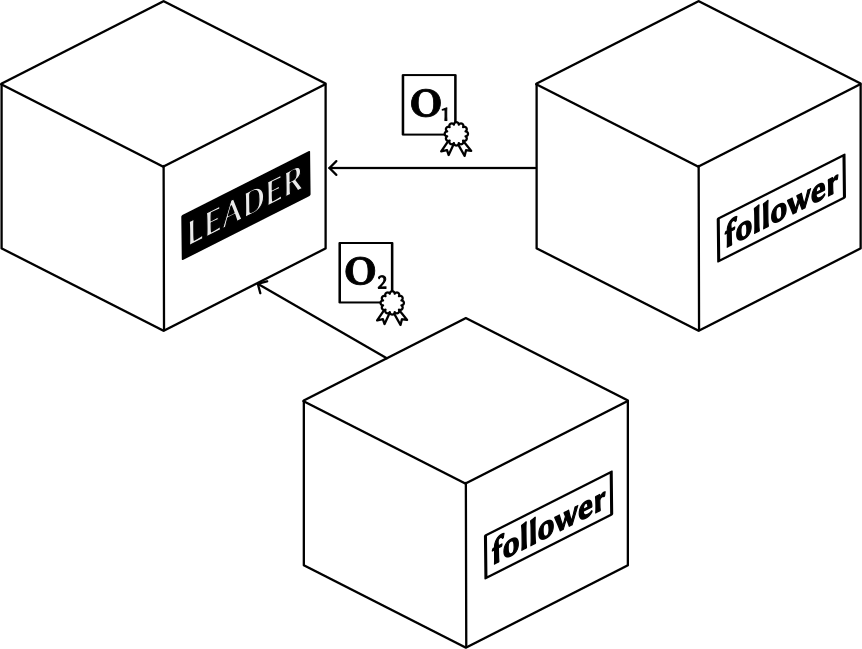
\includegraphics{/images/24-report-2.svg}
\end{figure}

If the leader receives at least \math{2f+1} observations, it distributes these signed (or \emph{attributed}) observations among the followers.
\begin{figure}[grayscale-diagram,medium-size]
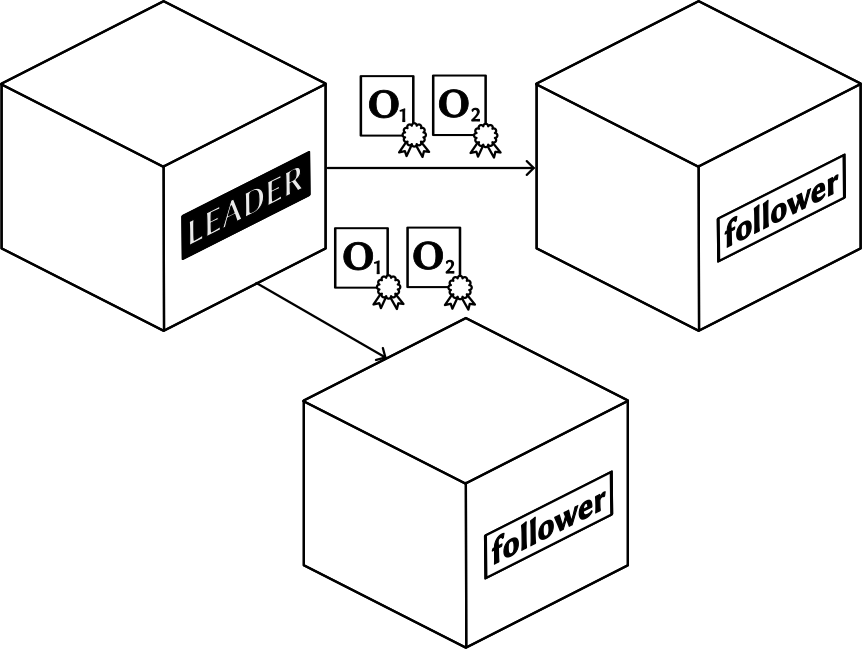
\includegraphics{/images/24-report-3.svg}
\end{figure}

Next, the followers distill attributed observations into a \emph{report}, sign it, and send it to the leader.
In the asset price example, the report is the median price.
The observation aggregation function must consider any \math{f} out of at least \math{2f+1} observations untrustworthy for the protocol to be byzantine-fault-tolerant.
For example, the asset price application must not pick one of the top or bottom \math{f} prices.
\begin{figure}[grayscale-diagram,medium-size]
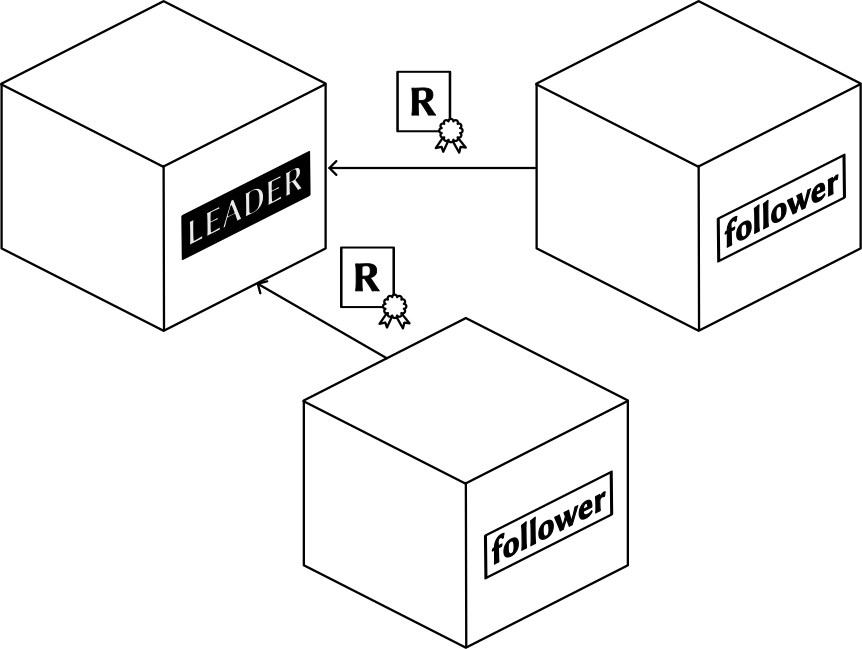
\includegraphics{/images/24-report-4.svg}
\end{figure}

If at least \math{f+1} followers signed the same report, the leader aggregates the report and the signatures into an \emph{attested} report and transmits it to all the followers.
\begin{figure}[grayscale-diagram,medium-size]
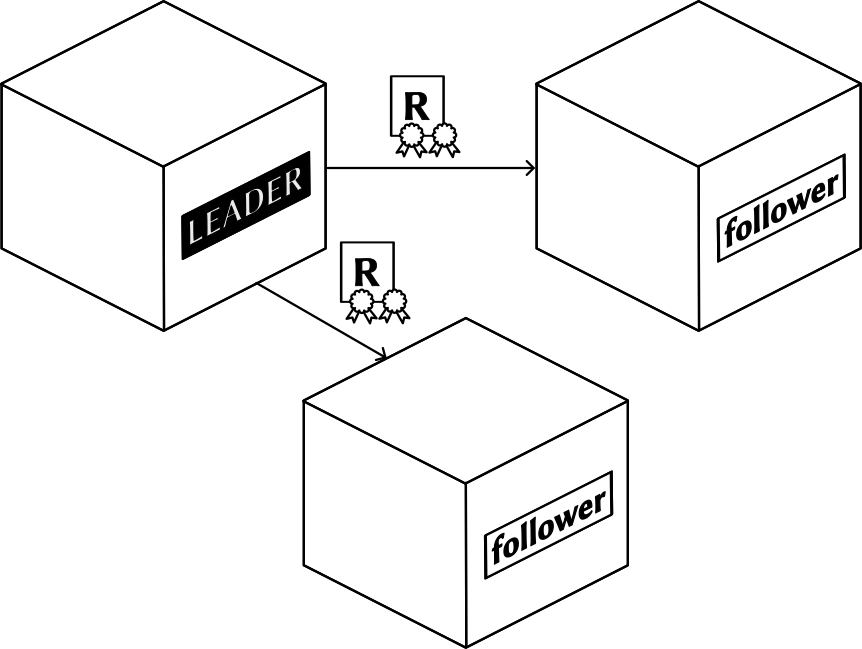
\includegraphics{/images/24-report-5.svg}
\end{figure}

Once the followers receive an attested report, they initiate the transmission algorithm.

\subsection{transmission}{Transmission}

The goal of the transmission algorithm is to record an attested report on the blockchain.

The algorithm has the following steps:
\begin{enumerate}
    \item The nodes check the aggregator contract's state and skip the transmission if the state matches the report data or deviates insignificantly.
    \item Every node sets a timer with a pseudo-random delay depending on the node's ranking in the current round.
    After the timer expires, the node rechecks the contract state to account for other nodes sending a transaction earlier.
    If the contract state is still stale, the node submits a blockchain transaction to update it.
    \item Once the aggregator contract receives an attested report, it validates the signatures, updates its state accordingly, and distributes rewards to the report signers and the transaction transmitter.
\end{enumerate}
\begin{figure}[grayscale-diagram,medium-size]
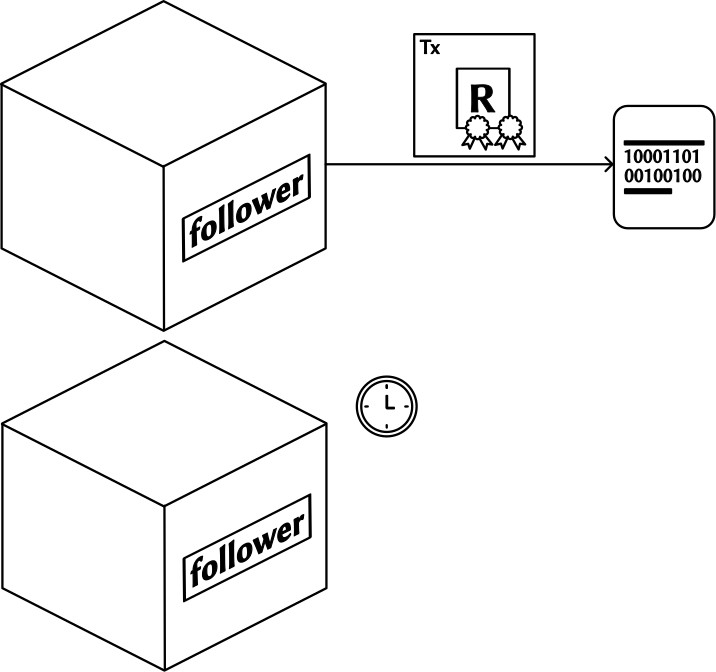
\includegraphics{/images/24-transmission.svg}
\end{figure}

The transmission algorithm guarantees the correctness and freshness of data on the blockchain but not the fairness of transmission rewards.
A malicious node can reap transmission rewards in every round if it ignores the randomized transmission schedule.
The aggregator contract owner can mitigate this issue by monitoring the transmission order and punishing misbehaving nodes.

\section{iterations}{Protocol version iterations}
\begin{itemize}
    \item \sc{ocr 1.0} specifically targeted data feeds for \sc{evm} blockchains.
    \item \sc{ocr 2.0} is a major iteration that introduced a plugin architecture, significantly extending the protocol's capabilities.
    This version also features reduced gas costs, a more secure \sc{p2p} networking stack based on \sc{tls1.3}, and better performance characteristics (lower latency, higher throughput).
    \item \sc{ocr 3.0} made the plugin interface more flexible, introduced the observation history chain, reduced the latency, and improved throughput using the report batching feature.
\end{itemize}

\section{resources}{Resources}

\begin{itemize}
    \item The \href{https://research.chain.link/ocr.pdf}{Chainlink Off-chain Reporting Protocol} whitepaper by Lorenz Breidenbach et al. describes the first protocol version in great detail and contains proofs of its security properties.
    \item The \href{https://github.com/smartcontractkit/libocr/blob/6359502d2ff1165c7e6b77b9eff2c5a46a7a4fbb/offchainreporting2plus/ocr3types/plugin.go#L94}{\sc{ocr3} plugin interface} documents the general flow and extention points.
    \item In the \href{https://youtu.be/XKiLkmwVaYA}{Looking under the hood of \sc{ocr} 2.0} video, Lorenz Breidenbach explains the protocol evolution and the plugin architecture.
    \item In the \href{https://youtu.be/VPVH3QCwc0U}{\sc{ocr3} protocol overview} video, Chrysa Stathakopoulou outlines the protocol structure and mentions features added in its third iteration.
\end{itemize}
\end{document}
